\chapter{The Exporter}
\label{ch:export}

%So far we have been working in a simplistic dependent language. The next step is to export our work in Tog into systems that are widely used for theory development and proofs. We start with Agda, as it is the one that resembles Tog the most. 

Generating the definitions of constructions from a theory presentation saves a lot of library development time, but having these definitions in a feature-rich language makes it even more useful. In this chapter we implement an automatic translator of the library theories and their related constructions to Agda and Lean. This part is related to the third research question from Section~\ref{sec:questions}. 
%and lean\ednote{lean is still being implemented} 

We study how different Agda and Lean are from Tog in Section~\ref{sec:beyongTog}. We discuss our design of an exporter in Section~\ref{sec:export_design}. The implementation in Haskell, the meta-language for Tog is disucssed in Section~\ref{sec:exporting_agda}. We compare our generated Agda code to the one in the Agda standard library~\cite{agda_stdlib} and discuss how close we can get to the standard library presentation in Section~\ref{sec:compasion_agda_stdlib}. 
%To assess how our approach scale up, we discuss how we extended the exporter to support lean, as a target language, in Section~\ref{sec:exporting_lean}. 
We wrap by a discussion in Section~\ref{sec:exporting:discussion}. 

\begin{comment}
One of the problems we highlight here is how design decisions lead to different presentations of the same theory, forcing developers to rewrite the same mathematical knowledge in different ways. In this chapter, we investigate the following question
\begin{itemize}
\item Given the tog abstract representation, can we export to formal systems with more complex meta theory and design decision. 
\end{itemize}
\end{comment}

\section{Beyond Tog}
\label{sec:beyongTog}
As an experimental small language, Tog lacks some features that are usually found in main stream ones. In this section we discuss these features 

\subsection{Universes}
Tog provides only one kind \lstmath{Set}. It does not support universe hierarchy, and so in tog \lstmath{Set : Set}. On the other hand, Agda and Lean has an infinite number of universes. This is expressed in Agda as 
\lstmath{Set$_{\text{n}}$ : Set$_{\text{n+1}}$} for any natural number $\text{n}$.\footnote{In Lean, the hierarchy is expressed as \lstmath{Type n : Type (n+1)} for any natural number \lstmath{n}.}
All the constructions we generate belong to the same level, except for relational interpretations, which describe a structure-preserving relation between two instances of the theory; see Section~\ref{sec:generation:relInterp}. In Tog, relational interpretations are records and the relation is a field of the record represented as 
\begin{togcode}
interp : A1 -> A2 -> Set
\end{togcode}
\noindent for types \lstmath{A1} and \lstmath{A2}, which are carriers of the two instances. 
A record with this field in Tog has a type \lstmath{Set} and therefore belong to universe level zero. When exported to Agda or Lean, its definition needs to have the type universe level 1.  

\subsection{Prelude Definitions}
The constructions we generate from theory presentations depend on Tog definition of \lstmath{Nat}, \lstmath{Fin}, \lstmath{Vec}, and \lstmath{lookup}. Tog does not support indexed types and defines \lstmath{Fin} as  
\begin{togcode}
data Fin (n : Nat) : Set where
  fzero : (m : Nat) (p : n == suc m) -> Fin n
  fsuc  : (m : Nat) (p : n == suc m) (i : Fin m) -> Fin n
\end{togcode}
\noindent This leads to a rather complicated definition of the \lstmath{lookup} function. 

On the other hand, Agda supports indexed types, has a simpler definition of \lstmath{Fin} and \lstmath{lookup}, and has these definitions in its standard library. Similarly, lean has types and functions for the same purposes, but different names.

\subsection{Equality Check in Pattern Matching}
One of the things we generate is a simplifier that uses axioms like \lstmath{e * x $\ \equiv\ $ x} to simplify expressions; see Section~\ref{sec:generation:simplifier}. 
In a theory that has a binary operation with an inverse and a unit, like \lstmath{Group}, a possible axiom is  
\begin{agdacode}
op x (inv x) ~$\equiv$~ e 
\end{agdacode}
\noindent which would give rise to a simplification rule. To perform this simplification, one needs to compare the two occurrences of \lstmath{x} for equality. While Tog accepts using the same variable name in pattern matching, and considers the two occurrences to be equal, Agda and Lean would not accept that code. Therefore, to perform the simplification, we need to compate them using decidable equality.

\subsection{Functions as Constructors}
In Section~\ref{sec:generation:staged} we discussed automatically annotating term languages to produce staged expressions. We discussed a problem related to how Tog represents constructors of a datatype. Tog does not allow passing constructors to higher order functions. Instead, we had to define a function corresponding to these constructors and pass it to the functions that lifts them to their staged versions. When exporting to Agda or Lean, we do not need to keep this trick.

\section{Exporter Design}
\label{sec:export_design}
The Tog definitions have all the information needed to mathematically present the concepts they are describing. The process of exporting these definitions from Tog to Agda or Lean can be seen as \emph{presenting} them in a way that the target language understands (type checks).

In the previous section, we discussed some of the misalignments between the presentations of concepts in Tog versus Agda or Lean. 
%Therefore, the exporter needs to do some preprocessing of the input Tog representation. 
The preprocessing manipulates the syntax tree to resolve these issues.  
%like the ones discussed in the previous section, which are common to both Agda and Lean, as well as ones that are specific to each language like the literal names. 
Afterwards, the exporter traverses the syntax tree and prints the output in the format accepted by the target language. Language specific keywords and options are specified using a configuration type. The design of the exporter is illustrated in Figure~\ref{fig:exporter_design}. 
\begin{figure}
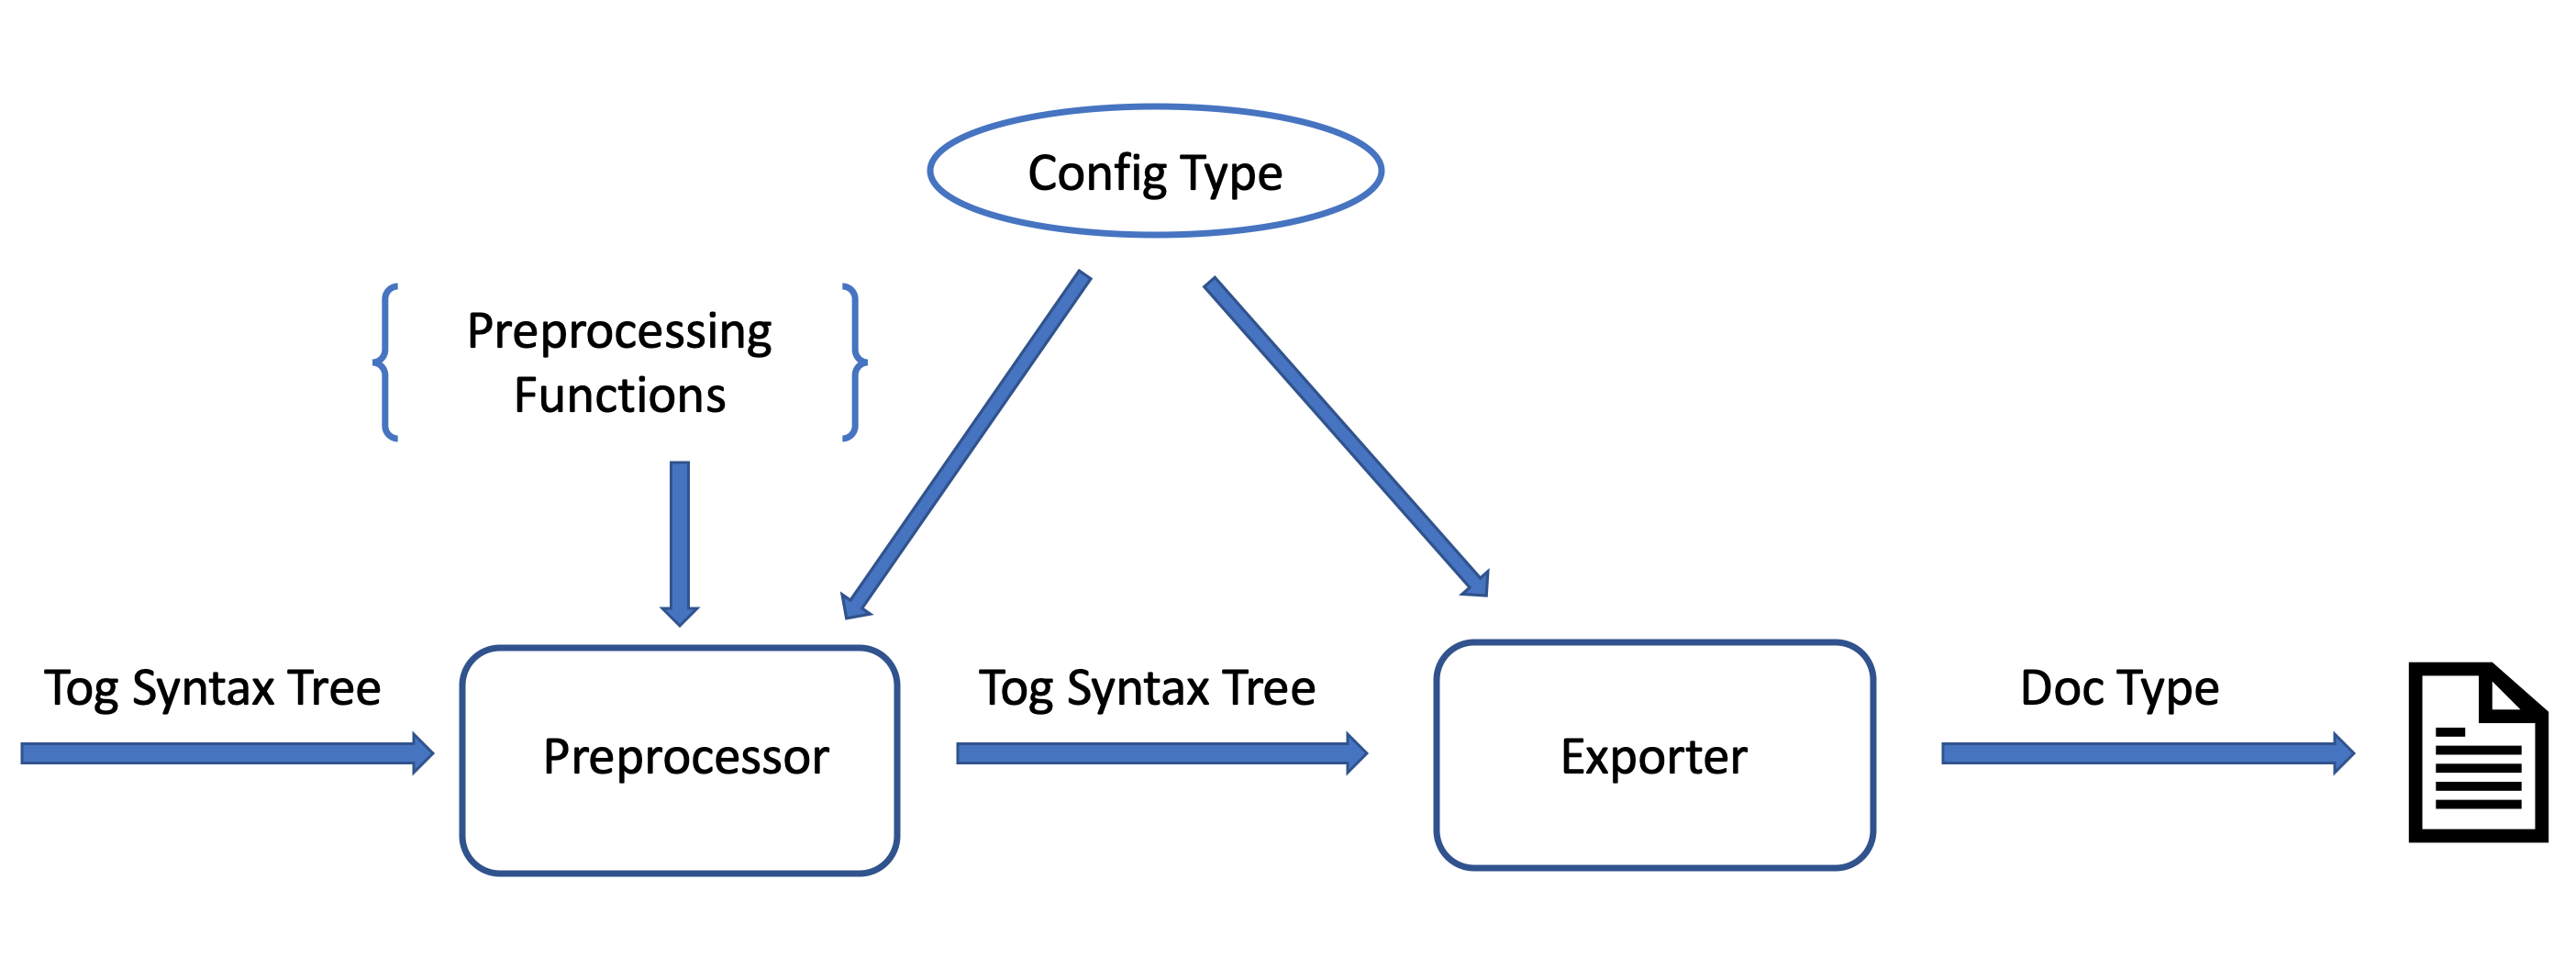
\includegraphics[scale=0.3]{figures/exporter_arch.png}
\caption{The design of the exporter.}
\label{fig:exporter_design}
\end{figure}

\section{Implementation}
\label{sec:exporting_agda}

We discuss our implementation of the design in Section~\ref{sec:export_design}. We start by discussing the preprocessing functions in Section~\ref{sec:exporting:challenges} showing how they solve the problems highlighted in Section~\ref{sec:beyongTog}. In Section~\ref{sec:impl:exporter} we introduce the \lstmath{Export} type class that performs that translation from the modified Tog syntax tree to the definitions of the target language. 

\subsection{The Preprocessor}
\label{sec:exporting:challenges}
The first stage of the exporter is to preprocess the Tog syntax tree to account for the issues discussed in Section~\ref{sec:beyongTog}. In this section, we discuss the manipulations performed by the preprocessor. 

\subsubsection{Universes}
To solve the universes problem, we provide the function \lstmath{universeLevel} which checks the fields of a record for a \lstmath{Set} type. If it finds one, it sets the type of the record to universe level 1, where the representation of the level is read from the config file. 
\begin{hscode}
universeLevel :: Config -> Fields -> Doc
universeLevel conf flds =
  text ~$\$$~
    if elem "Set" ~$\$$~ everything (++) (mkQ [] (\ (Name (_,x)) → [x])) flds
    then (level1 conf) else (level0 conf)    
\end{hscode}
The function \lstmath{universeLevel} is called every time a record header is printed. 

\subsubsection{The Prelude}
Exporting the prelude definitions is done differently than exporting the generated code. The configuration type includes information about how they are processed, via the field
\lstmath{prelude_includes :: Either FilePath ([ImportDecl],[String])}. If the value has the type \lstmath{FilePath}, then the provided includes the definitions of the prelude. Otherwise, the configuration provides a list of import declarations, to be added at the beginning of the prelude module, and a list of the names of definitions to be exported. 
For example, the \lstmath{prelude_includes} of the Agda configuration is 
\begin{hscode} 
 Right (["open import Agda.Builtin.Equality",
         "open import Agda.Builtin.Nat",
         "open import Data.Fin",
         "open import Data.Vec"]
      ,["Prod","Wrap","Stage","CodeRep","uncode","code","run",
        "Choice","Comp","Staged","expr","const",
        "stage0","stage1","stage2","codeLift1","codeLift2"])   
\end{hscode} 

The imports for modules other than prelude is defined using the \lstmath{imports} config declaration. 

The function \lstmath{mkImport} creates import declarations for all modules based on the information retrieved from the configuration. \lstmath{import_}, \lstmath{open_}, and \lstmath{openimport} are the keywords to import, open, or open-import a module in the target language. The function reads the names of these modules and created instances pd \lstmath{Decl} using the corresponding constructors. 
\begin{hscode}
mkImports :: Config -> [String] -> [Decl]
mkImports conf imprts =
  let getNames prefix =
        if prefix == "" then [] 
        else removePrefix conf ~$\$$~ filter (isPrefixOf prefix) imprts
       createImport x = ImportNoArgs ~$\$$~ mkQName x
  in (map (Import . createImport) ~$\$$~ 
         (getNames ~$\$$~ import_ conf) \\ (getNames ~$\$$~ openimport conf))
  ++ (map (OpenImport . createImport) ~$\$$~ getNames (openimport conf))
  ++ (map (Open . mkQName) ~$\$$~
         (getNames ~$\$$~ open_ conf) \\ (getNames ~$\$$~ openimport conf))
\end{hscode} 

When importing functions, the order of their inputs may be different than that used when calling the same function in Tog. This is the case with the definition of \lstmath{lookup} in Agda versus Tog where the two arguments are flipped. In Lean the function name is \lstmath{nth} and the arguments are also flipped with respect to the tog definition. To solve this problem, every target exporter has a function \lstmath{callFunc} that adjusts the call to the function. The one for agda is: 
\begin{hscode}
callFunc :: Expr -> Expr
callFunc a@(App [nm,_,a2,a3]) =
  if (getArgName nm == "lookup") then App [nm,a3,a2] else a
callFunc e = e
\end{hscode}
\noindent \lstmath{callFunc} is called before every function application is exported. Therefore, it can be easily extended to adjust calls to any function. 

\subsubsection{Simplifier}
One of the constructions that can be generated is decidable equality. In case they are generated, they can be used to check for equality of variables. Since we do not generate them, we remove simplification rules that includes two occurrences of the same variable name in the pattern. 

\subsubsection{Functions as Constructors}
Not allowing constructors to be passed to higher order functions resulted in creating a function declaration for every constructor of term languages during the generation phase of the interpreter. 
The function \lstmath{constructorsAsFunctions} removes these generated functions, as they are not needed for Agda or Lean. The function is defined as follows: 
\begin{hscode} 
constructorsAsFunctionsHelper :: Config -> [Constr] -> [Decl] -> [Decl] 
constructorsAsFunctionsHelper conf cs decls =
  let cnames = map getConstrName cs
      toFindNames = map opDeclToFuncName cnames 
      mapping = zip toFindNames cnames
  in if(constructors_as_functions conf) then decls 
      else foldrenConstrs mapping ~$\$$~ 
               filter (\d -> not  ~$\$$~  elem (declName d) toFindNames) decls     
\end{hscode} 
\noindent \lstmath{cnames} is a list of the names of the constructors and \lstmath{toFindNames} is a list of their corresponding functions. \lstmath{filter} is used to remove these definitions from the list of declarations of the module. \lstmath{foldrenConstrs} is then used to substitute their names with the names of the corresponding constructors. 

\subsubsection{Field Names}
Another misalignment between Tog, Agda, and Lean is what names can be used for fields. Agda does not allow them to be numbers. Lean does not accept numbers or symbols like \lstmath{+, *, \|>, <\|}. 
We provide a function \lstmath{replace} that is called before any \lstmath{Name} is printed. The \lstmath{replace} function for Agda is: 
\begin{hscode}
replace :: String -> String
replace nm =
  let pieces = splitOn "_" nm
      cond = \x -> if (x == "0" || x == "1") then x ++ ~$_i$~ else x
      postProcess lst = (head lst) : (map ("_"++) ~$\$$~ tail lst)
  in concat ~$\$$~ postProcess ~$\$$~ map cond pieces 
\end{hscode}
A name which is just \lstmath{0} or \lstmath{1} is concatenated with a suffix \lstmath{$_i$}. The suffix is also added if the \lstmath{0} or \lstmath{1} is part of a name, but is separated by \lstmath{_}. This accounts for the naming convention of the MathScheme library for axioms. 

\subsection{The Exporter} 
\label{sec:impl:exporter}
The type class, \lstmath{Export}, prints the Tog definitions in a form accepted by the target language, whose type checker is then called on them. 
\begin{hscode}
class Export a where
  export :: Config -> a -> Doc  
\end{hscode}
The \lstmath{Config} type is used to describe the configuration of each language. It contains details about language specific properties or pieces of syntax. 
%Based on the users' choice of the export language, the exporter loads the corresponding \lstmath{Config} instance and preprocessing functions.  
For every type in the Tog AST, we create an instance for the \lstmath{Export} class.
We use the Haskell pretty printer provided by \lstmath{Text.PrettyPrint.Leijen}, which is an implementation of the pretty printer described in~\cite{wadler2003prettier}. 

\subsubsection{The Pretty Printer}
In~\cite{wadler2003prettier}, an algebra for defining pretty printers is introduced, based on $6$ primitives: 
\begin{hscode}
(<>) :: Doc -> Doc -> Doc 
empty  :: Doc 
text :: String -> Doc 
line :: Doc 
nest :: Int -> Doc -> Doc 
layout :: Doc -> String 
\end{hscode}
\noindent where \lstmath{Doc} is the type of a document. The \lstmath{(<>)} operation concatenates two documents. It is an associative operation with \lstmath{empty}\footnote{\cite{wadler2003prettier} refers to \lstmath{empty} as \lstmath{nil}.} being its right and left unit. 
%\begin{comment}
On top of these primitives, we have used the following functions provided by the 
\lstmath{Text.PrettyPrint.Leijen}. 
\begin{itemize}
\item \lstmath{(<+>)} : concatenates two \lstmath{Doc} instances with a space between them. 
\item \lstmath{(<$\$\$$>)} : concatenates two \lstmath{Doc} instances with a \lstmath{line} in between them. 
\end{itemize}
%\end{comment}

\subsubsection{The Exporter Type Class}
We present here some of the interesting instances of the \lstmath{Export} type class\footnote{The full code is available at: \url{https://github.com/ysharoda/Deriving-Definitions/blob/7e19c3c7d6240d7ff228a91c6c32d1914c483195/src/Tog/Exporting/export.hs}.}. 
Our generator defines every theory along with its generated constructions in a  \lstmath{Module}. Exporting a \lstmath{Module} is described by the following instance 
\begin{hscode} 
instance Export Module where
  export conf (Module nm params decls) =
    export conf imprts <~$\$\$$~>
    text (m1 conf) <+> export conf nm <+> text (m2 conf) <+> 
    export conf params <+> text (m3 conf (isEmpty decls)) <~$\$\$$~>
    (indent 2 ~$\$$~ export conf defs) <~$\$\$$~>
    moduleEnd conf nm 
    where (imprts,defs) = split conf decls
          isEmpty (Decl_ []) = True
          isEmpty _ = False 
\end{hscode} 
In order to write one exporter with two target languages, we need to investigate the commonalities and differences between them. The first obvious difference is the keywords used. The exporter reads the keywords of the target language from its configuration. 
On the level of modules, we use the configuration fields \lstmath{m1, ..., m4} as follows 
\begin{lstlisting}
            m1 nm m2 params m3 
            ...
            m4
\end{lstlisting}
All configuration fields are printed using the \lstmath{text} function. 

Another difference between our two target languages is the structure of their module system. The general structure of modules in Agda and Lean is 

\begin{tabular}{p{18em} p{10em}}
\begin{agdacode} 
module nm params where 
  import ...
  ... 
~$\newline$~        
\end{agdacode}  
&
\begin{leancode}
import ...
section nm 
  ... 
end nm 
\end{leancode}
\end{tabular}

%Agda modules (on the left) uses the keywords \lstmath{module} and \lstmath{where} to define the module, while lean (on the right) uses \lstmath{section} and \lstmath{end} to mark the beginning and end of a module. The keywords specific to the target language of the exporter are read from its instance of the \lstmath{Config} type. 

The configuration of each language specifies the position of the import declarations. The function \lstmath{split} checks the configuration for this information and accordingly splits the module declarations into those to be printed before its header (if any), and those who are part of the module. 

The  \lstmath{moduleEnd} function checks if the module needs to be closed with any keywords, and whether the name of the module needs to be included as in lean. The \lstmath{export} function is called on the components of the module, which are the name (\lstmath{nm}), the parameters (\lstmath{params}) and the declarations within the module (\lstmath{decls}). 

The parameters of a module are represented as \lstmath{[Binding]}, which can be hidden or explicit. Exporting the binding is done by calling \lstmath{export} on its arguments and type expression.  
\begin{hscode}
instance Export Binding where
  export conf binds =
    let arguments as = hsep ~$\$$~ map (export conf) as
        binding x =  
          arguments (getBindingArgs x) <+> text (bind_of_type conf) 
          <+> export conf (getBindingExpr x)
    in case binds of
      Bind  _ _ -> parens ~$\$$~ binding binds
      HBind _ _ -> braces ~$\$$~ binding binds

\end{hscode}
Every \lstmath{Binding} consists of a set of arguments of type \lstmath{Arg} that defines the variables of the binding. the function \lstmath{getBindingExpr} returns the type of those binding arguments. 

The body of the module consists of declarations \lstmath{[Decl]}. Exporting each of these declarations is straight forward by calling the \lstmath{export} function on its components. Function definitions in Agda are declared by writing the function names for every pattern, while in Lean guards are used to declare the different patterns. 
\newline
\begin{tabular}{p{18em} p{10em}}
\begin{agdacode} 
f : ~$binds-list \to type-expr$~   
f x0 .. xn = ... 
...    
\end{agdacode}  
&
\begin{leancode}
def f ~$binds-list : type-expr$~ 
| x0 ... xn = ... 
... 
\end{leancode}
\end{tabular}
\newline
If the function name is part of the definition, the configuration is set to be \lstmath{"fname"}. The function \lstmath{funcHeader} takes care of this case. 

The instance of \lstmath{Export} for \lstmath{Decl} is:  
\begin{hscode}
instance Export Decl where
  export conf (TypeSig sig) = export conf sig 
  export conf (FunDef nm ps body) =
    funcHeader (f5 conf) nm <+> (hsep ~$\$$~ map (export conf) ps) 
    <+> text (f6 conf) <+> export conf body <+> text (f7 conf)
    where funcHeader flag fname = 
            if flag =="fname" then export conf fname else text flag    
  export conf (Data nm ps body) =
    text (d1 conf) <+> export conf nm <+> text (d2 conf) 
    <+> export conf ps <+> text (d3 conf) <+> export conf body 
    <+> openDatatype conf nm
  export conf (Record nm ps body) =
    text (s1 conf) <+> export conf nm <+> text (s2 conf) 
    <+> export conf ps <+> text (s3 conf) <+> export conf body 
  export conf (Open imp) = text (open_ conf) <+> export conf imp
  export conf (Import imp) = text (import_ conf) <+> export conf imp
  export conf (OpenImport imp) = 
    text (openimport conf) <+> export conf imp
  export conf (Module_ m) =
    linebreak <+> export conf m  <+> linebreak 
  export _ _ = empty
\end{hscode}

With instances of \lstmath{export} for every type in the tog abstract syntax, a single call to \lstmath{export} on the top level module of the tog library generates the equivalent Agda definitions\footnote{The generated files available at:~\url{https://github.com/ysharoda/Deriving-Definitions/tree/master/Library/generated/mathscheme-agda}.}.

\section{Comparison With Agda Standard Library}
\label{sec:compasion_agda_stdlib}
%Some of the constructions generated in this work is part of the agda standard library and some are not. 
We compare the the definitions that we generate in Agda to those in its standard library, highlighting how close we can get to them. 
%look at our generated theories and constructions and compare them with the ones that agda provides in its standard library, highlighting how close we can get to them. 

Algebraic structures in Agda are unparameterized records. For example, \lstmath{Monoid} is defined as\footnote{source:\url{https://github.com/agda/agda-stdlib/blob/84dcc85a8c6ee258d8a00f7137b9db399cdb62da/src/Algebra/Bundles.agda}.}:
\begin{agdacodelnos}
record Monoid c ~$\ell$~ : Set (suc (c ~$\sqcup$~ ~$\ell$~)) where 
  infixl 7 _~$\bullet$~_
  infix 4 _~$\approx$~_
  field 
   Carrier : Set c 
   _~$\approx$~_ : Rel Carrier ~$\ell$~ 
   _~$\bullet$~_ : Op~$_2$~ Carrier 
   ~$\varepsilon$~ : Carrier 
   isMonoid : IsMonoid _~$\approx$~_ _~$\bullet$~_ ~$\varepsilon$~ 
   
   open IsMonoid isMonoid public
   
   semigroup : Semigroup _ _
   semigroup = record { isSemigroup = isSemigroup }
   
   open Semigroup semigroup public using (rawMagma; magma)
   
   rawMonoid : RawMonoid _ _
   rawMonoid = record { _~$\approx$~_ = _~$\approx$~_; _~$\bullet$~_ = _~$\bullet$~_; ~$\varepsilon$~ = ~$\varepsilon$~}
\end{agdacodelnos}
\noindent The definition of \lstmath{Monoid} is universe polymorphic, \lstmath{c} and \lstmath{$\ell$} refer to the universe levels of the carrier and the equality relation. 
Line $2$ and $3$ define notation for infix binary symbols, specifying their precedence. Line $5$ defines the carrier of the \lstmath{Monoid} structure. The carrier belongs to universe level \lstmath{c}. 
Line $6$ defines the equality used to compare terms of \lstmath{Monoid}. Since the algebraic hierarchy in Agda's standard library is based on setoids, equality is explicitly defined for every algebraic structure. 
Lines $7$ and $8$ defines the function symbols of \lstmath{Monoid}. The axioms of \lstmath{Monoid} are defined by instantiating the \lstmath{IsMonoid} record, which can be seen as an unbundled variation of the definition of \lstmath{Monoid}. Given the function symbols of \lstmath{Monoid}, the \lstmath{IsMonoid} record declares the axioms they need to satisfy. \lstmath{IsMonoid} is defined as: 
\begin{agdacode}
record IsMonoid (~$\bullet$~ : Op~$_2$~) (~$\varepsilon$~ : A) : Set (a ~$\sqcup$~ ~$\ell$~) where 
  field 
   isSemiring : IsSemiring ~$\bullet$~ 
   identity : Identity ~$\varepsilon$~
     
  open IsSemigroup isSemigroup public
     
  identity~$^l$~ : LeftIdentity ~$\varepsilon$~ ~$\bullet$~ 
  identity~$^l$~ = proj~$_1$~ identity  
  identity~$^r$~ : Rightdentity ~$\varepsilon$~ ~$\bullet$~ 
  identity~$^r$~ = proj~$_2$~ identity           
\end{agdacode}

\noindent The instance of \lstmath{IsMonoid}, in the \lstmath{Monoid} definition, is opened in line $11$ so its declarations can be accessed without qualifying their names. 
Lines $13$ and $14$ defines a backward morphism from \lstmath{Monoid} to \lstmath{Semigroup}. This \lstmath{semigroup} function defines a \lstmath{Semigroup} instance for every \lstmath{Monoid} one. 
Lines $18$ and $19$ extracts an instance of type \lstmath{RawMonoid} for every instance of type \lstmath{Monoid}. 

The flattener described in Chapter~\ref{ch:library} computes flat theories parametrized over the carrier. By comparing the two representations we find that they mainly differ in three aspects that we detail in the following sections. 
\subsection{Predicate Style Presentations}
A predicate style presentation for a theory $\Gamma = (\mathcal{S},\mathcal{F}, \mathcal{E})$ splits its declarations into two records. The \lstmath{is$\Gamma$} record has the sort and function symbols as parameters, while having the axioms as record fields. The second record, $\Gamma$, is an unparametrized record. 

Starting from flattened theories, the following function generates \lstmath{is$\Gamma$} 
\begin{hscode}
isX :: GTheory -> GTheory
isX (GTheory constrs _) =
  let newWaist = length (notAxiom constrs) 
  in GTheory (notAxiom constrs ++ axiom constrs) newWaist
\end{hscode}
\noindent The waist of a theory reflects the number of its parameters. The \lstmath{newWaist} is set to be the number of declarations that are not axioms. 

The definition of the theory \lstmath{$\Gamma$} is changed to include an \lstmath{is$\Gamma$} instance.  
\begin{hscode}
adjustTheory :: Name_ -> GTheory -> GTheory
adjustTheory thryName (GTheory constrs wst) =
  let isXName = "Is"++thryName
      fsyms = notAxiom constrs
      fsymNames = map (\ (Constr (Name (_,nm)) _) -> nm) fsyms
      processName n = if elem n ["+","-","*"] then "("++n++")" else n 
      callIsX = [Constr (mkName ~$\$$~ "is"++thryName)
                     (App ~$\$$~ (mkArg isXName) 
                          : (map (mkArg . processName) fsymNames))]
  in GTheory (fsyms ++ callIsX) wst 
\end{hscode} 
These functions produce the following definitions for \lstmath{Monoid}: 
\begin{agdacode}
record IsMonoid (A  : Set ) (op  : (A  ~$\to$~ (A ~$\to$~ A ))) (e  : A ) 
                : Set where
  constructor IsMonoidC
  field
   lunit_e : ({x  : A }  ~$\to$~ (op e x ) ~$\equiv$~ x )
   runit_e : ({x  : A }  ~$\to$~ (op x e ) ~$\equiv$~ x )
   associative_op : ({x y z  : A }  ~$\to$~ 
            (op (op x y ) z ) ~$\equiv$~ (op x (op y z ) )) 

record Monoid (A  : Set )  : Set where
  constructor MonoidC
  field
   op : (A  ~$\to$~ (A  ~$\to$~ A ))
   e : A 
   isMonoid : (IsMonoid A op e ) 
\end{agdacode}
There are three main differences between the \lstmath{IsMonoid} in the Agda standard library and the one generated here: 
\begin{itemize}
\item The definition provided by the standard library does not have the carrier as a parameter. The carrier is still part of the context, but is declared as an implicit argument to the parent module. 
\item The standard library represents axioms as instances of records, like \lstmath{IsSemiring} and \lstmath{Identity}. Automating this introduces a layer of complexity that we discuss in Section~\ref{subsec:agda:modelMorphisms}. 
\item Library definitions are universe polymorphic. Tog does not have universes and all our generated records have the type \lstmath{Set}. 
\end{itemize} 
%The record \lstmath{Monoid} have the same differences. Due to the absence of universe support in Tog, we prefer to keep the generated \lstmath{Monoid} record parametrized over the carrier. 

\subsection{Setoids Based Presentations}
\label{subsec:setoid-based-pres}
The algebraic hierarchy in Agda are defined over setoids, i.e. every carrier set is equipped with its own equality. 
The theory of setoid can be obtained from the \lstmath{Carrier} theory using the extension combinator 
\begin{togcode}
Setoid = extend Carrier {eq : A -> A -> Set}
\end{togcode}
In our development, the equality used to represent the equations is Tog's underlying propositional equality. It is part of the meta theory and is not reflected in the theories or the morphisms of the graph. Therefore, switching to a different equality would require doing that on the meta theory level. 

On the other hand, if we start with a graph developed with equality at the theories level, using setoids, one can switch to built-in equality by substitution. 


% The data being manipulated in this work is theories in equational logic. The theories of algebra that we consider in this work are first order equational theories, i.e.: all the axioms are equations.

%The problem becomes changing all the axioms to be based on \lstmath{eq} instead of the tog equality. Tog equality is part of the meta thoery, tog, and is not part of any morphism, i.e.: cannot be mapped to \lstmath{eq} to adjust how the axioms look like. \ednote{TBD: how to handle this?}

%On the presentation level, this means that every theory would have one more declaration for the equality, as well as congruence axioms for all its function symbols. 

\subsection{Backwards Morphisms} 
\label{subsec:model-morph}
\label{subsec:agda:modelMorphisms}
The definition of \lstmath{Monoid} in the Agda standard library includes backward morphisms to  \lstmath{semigroup} definition that given a specific monoid would extract the semigroup structure of it. Our theory presentation does not have this reference. The information to generate these model morphisms is present in the theory graph. The graph has a theory presentation morphism between \lstmath{Semigroup} and \lstmath{Monoid}, which triggers a backwards morphism from \lstmath{Monoid} to \lstmath{Semigroup}. It is worth mentioning that a mechanism to generate these morphisms in our setup will not, in all cases, produce the same model morphisms as the one in the Agda standard library. In this case, we are depending on the structure of the graph which is different than the one in Agda's library. We leave the presentation of morphism information in Agda or Lean as future work. 

%\section{Exporting to Lean}
%\label{sec:exporting_lean}

\section{Comparing with Lean's Mathlib}
\lstmath{Monoid} is defined in Mathlib as follows\footnote{source:\url{https://github.com/leanprover-community/mathlib/blob/bc94d05242714263947fa485f3b64b911bb84faf/src/algebra/group/defs.lean}.}: 
\begin{leancode} 
@[ancestor semigroup has_one]
class monoid (M : Type u) extends semigroup M, has_one M :=
  (one_mul : ~$\forall$~ a : M, 1 * a = a) (mul_one : ~$\forall$~ a : M, a * 1 = a)
\end{leancode} 
The declaration \lstmath{@[ancestor semigroup has_one]} defines \lstmath{semigroup} and \lstmath{has_one} as the ancestors of \lstmath{monoid}. In a theory graph model, this means that an identity morphism exists between them. Note that the \lstmath{has_one} class is the representation of a class with one point, which we have referred to as \lstmath{Pointed}. 
Similar to the discussion we provided in Section~\ref{subsec:model-morph}, the information about the hierarchy is available in the graph we construct. Our current implementation does not export this information, and we leave it for future work. 

\section{Discussion}
\label{sec:exporting:discussion}
The idea of exporting from one language to another has been discussed various times, as we show in Section~\ref{sec:relwork:automation}. Our work take advantage from the fact that we export from a small language, and therefore the source syntax tree is small and can be manipulated easily.  
%Having a minimal source language gives us the opportunity to add design decisions without having to observe how it affects the multiple other features that would be present in a feature-rich language. That makes the export process easier to manage. 

As in Section~\ref{sec:generation:discussion}, we noted here that some missing features in Tog makes the exporting process a bit harder, like universes and indexed types. It is hard to decide which features are needed for a core language that fits our purpose. This is one way our work can be extended. We suggest studying theorem provers as a program family, capturing their commonalities and variabilities via techniques like feature models~\cite{czarnecki2000generative}. If we have this model, one can write a staged exporter to different languages in the model, similar to what is explained in~\cite{stagedConfig}. 

%The theory graph organization structure is useful to add model morphisms has proven useful in the exporting process. The fact that the morphisms carry information about It made it possible to add design decisions, like exporting to the setoids-based graph, and to add the model morphisms as we discussed in Section has also made it possible to incorporate model definitions, as we discuss in Section~\ref{subsec:model-morph}. 

\begin{comment}
Our algorithms generate record definitions, inductive data types and functions. We study how those three constructs look like in Agda. 

%\section{Record Definitions}
A record in Tog is has the type \lstmath{Decl} and is created using the \lstmath{Record} constructor as follows 
\begin{hscode}
Record Name Params RecordBody
\end{hscode}
The parameters are either empty or contains \lstmath{[Binding]}, as discussed in \ref{ch:tog}. \lstmath{RecordBody} contains information about the kind of the record, its constructor, and the fields it contains. A simplified view of the fields is \lstmath{[Constr]}. 

A record in Agda consists of 
\begin{itemize}
\item the keyword \lstmath{record}
\item the name of the type 
\item list of parameters surrounded by parenthesis  
\item A semicolon that seperates the name and params from the type 
\item the keyword \lstmath{where}
\item 
\end{itemize}
\end{comment}


